%!TEX root = ../main.tex
%%%%%%%%%%%%%%%%%%%%%%%%%%%%%%%%%%
% Links:
%
% Difficulty: Companies: 
%%%%%%%%%%%%%%%%%%%%%%%%%%%%%%%%%%


%\begin{figure} \centering 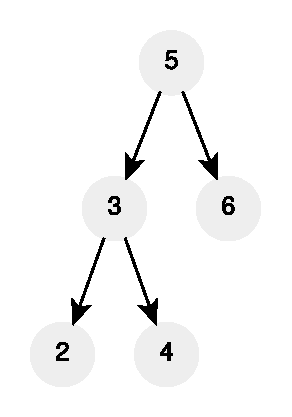
\includegraphics[width=\textwidth]{sources/max_manhattan/images/example1}
%   \caption[Sample short cpation]{Sample Caption}. \label{fig:max_manhattan:example1} \end{figure}

\chapter{Max in manhattan neighborhood$^{K}$}
\label{ch:max_manhattan}
\section*{Introduction}
This chapter discussed a very interesting problem that is based on the concept of the
\textit{Manhattan distance} \footnote{Also known as \textit{taxicab distance}.}
which is as the name suggest an alternative way to measure distances that
is particularly useful in real life. Imagine you need to measure the distance between two points in
a map. You can use the old and good Euclidean distance and come up with a number that in real life
is not going to be super helpful unless you are able to fly. This is because that number is not
going to tell you the actual distance you need to cover if you want to get to your destination my
moving on land. For instance, what is the distance between the Empire state building and Times
Square in New York? If you are not naturally equipped with wings than all you do is to jump on a car
or a cab or a bike and follow the grid pattern of streets of Manhattan and you would have to
probably cover around 15 blocks north and 3 south (See Figure
\ref{fig:max_manhattan:distance_manhattan}). The idea of measuring the distance by only counting the
number of steps we take the north-south, or west-east directions underlies what is known as the
taxicab distance. In this framework the distance is not represented as a straight line going from
point A to point B (like it would for the Euclidean distance) 
but it is a zig-zagged sequence of vertical and horizontal segments, representing movements along the north-south and east-west axis.
Therefore, the formula for measuring the taxicab distance is all about measuring length of the horizontal and verical
segments. The formula for measuring the manhattan distance in Equation
\ref{eq:max_manhattan:distance_formula}.
\begin{equation}
	d = |x_1-x_2|+|y_1-y_2|
	\label{eq:max_manhattan:distance_formula}
\end{equation}

The problem in this chapter will challenge you to find, for each cell of a given matrix,
the largest value in any cell sitting at a Manahtann distance below a certain threshold.

\begin{figure}
	\centering
	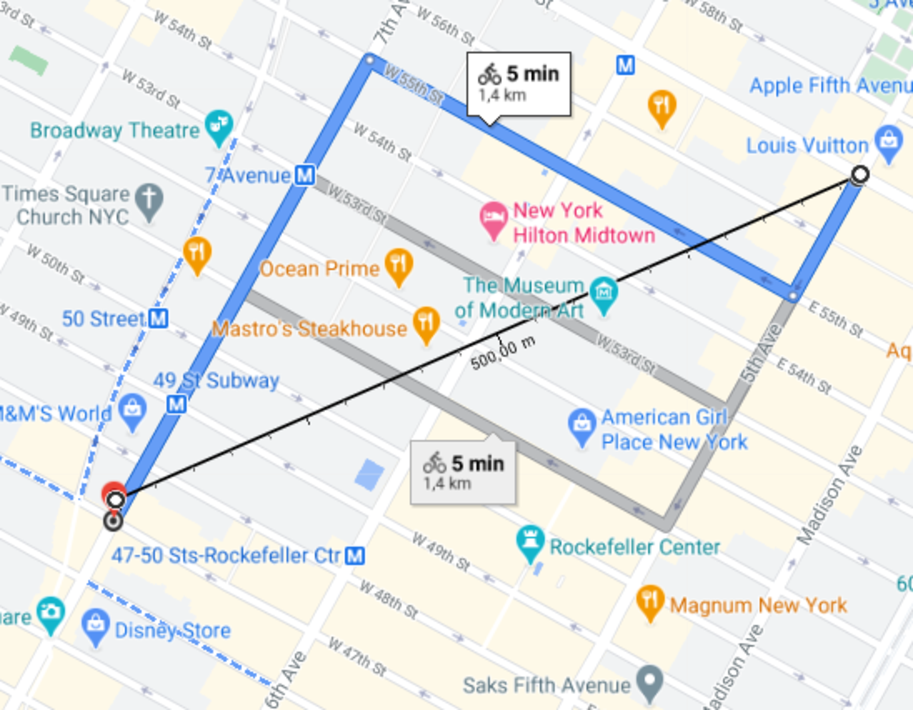
\includegraphics[width=\textwidth]{sources/max_manhattan/images/distance_manhattan2}
	\caption[Taxicab distance from times square to the trump tower]{Taxicab distance from times
	square to the Trump's tower. Notice that the black straight-line is depicting the Euclidean distance, 
	and that the latter is shorter than the actual taxicab distance between  the two points.}
	\label{fig:max_manhattan:distance_manhattan}
\end{figure}

\section{Problem statement}
\begin{exercise}
\label{example:max_manhattan:exercice1}
Write a function that given \begin{enumerate*}
	\item a matrix I of $n$ rows and $m$ columns and
	\item  an integer $K > 0$
\end{enumerate*}
returns a new matrix $M$ of size $n \times m$ where $M[i][j]$ contains the maximum value among the
elements in the manhattan neighborhood of size $K$ for the cell $(i,j)$.
The Manhattan neighborhood of size $K$ for a cell $(i,j)$ is composed of all cell $(p,q)$ such that:
\begin{equation}
	N(i,j, K) = \{(p,q) | |i-p|+|j-q| \leq K\}
	\label{eq:max_manhattan:neighbood_equation}
\end{equation}


\end{exercise}
	%example1
	\begin{example}
		\label{example:max_manhattan:example1}
		\hfill \\
		Given: $I=
		\begin{bmatrix}
		  1 & 2 & 3  \\
		  4 & 5 & 6  \\
		  7 & 8 & 9  
		\end{bmatrix}
	  $
  and $K=1$ the function return $I=
  \begin{bmatrix}
	  4 & 5 & 6  \\
	  7 & 8 & 9  \\
	  8 & 9 & 9  
	\end{bmatrix}
$
		
	\end{example}

	%example2
	\begin{example}
		\label{example:max_manhattan:example2}
		\hfill \\
		Given: $I=
		\begin{bmatrix}
		  1 & 2 & 3  \\
		  4 & 5 & 6  \\
		  7 & 8 & 9  
		\end{bmatrix}
	  $
  and $K=2$ the function return $I=
  \begin{bmatrix}
	  7 & 8 & 9  \\
	  8 & 9 & 9  \\
	  9 & 9 & 9  
	\end{bmatrix}
$
		
	\end{example}




\section{Clarification Questions}

\begin{QandA}
	\item 
	\begin{answered}
		\textit{}
	\end{answered}
	
\end{QandA}

\section{Discussion}
\label{max_manhattan:sec:discussion}

\subsection{Brute-force}
\label{max_manhattan:sec:bruteforce}
%You can optimize by only using N*M*2 space . see solution 2
This problem can be quite easily tackled by using a bruteforce approach that is basically finding the answer 
by blindly calculating the answer for each cell. 
All is necessary to find the answer for the cell $(i,j)$ is to find the maximum among the cells that are 
at a Manhattan distance of at most $K$ from it (the cells that are part of the Manhattan neighborhood of size $K$).
Figure \ref{fig:max_manhattan:neighborhood} shown an example of such neighborhood where the numbers inside the
cells represent the distance from the cell $(i,j)$ at the center. 
Given a cell $(i,j)$, figuring out exactly which cells are part of the neighborhood and which are not
is not particularly difficult but is definitely not trivial. 
Instead of coming up with a way of generating such list, it is easier to loop over all the cells within
a square of size $2K$ having cell $(i,j)$ at its center, and to ignore the ones that do not satisfy Equation \ref{eq:max_manhattan:neighbood_equation}.
Because both 
\begin{enumerate*}
	\item the number of cells in the neighborhood and 
	\item the number of cell in such square
\end{enumerate*} is quadratic in $K$, 
then, asymptotically speaking, the additional work required by visiting cells that are not part of the neighborhood
does not really make any difference. Listing \ref{list:max_manhattan:bruteforce} shows an implementation of such idea. 
\begin{figure}
	\centering
	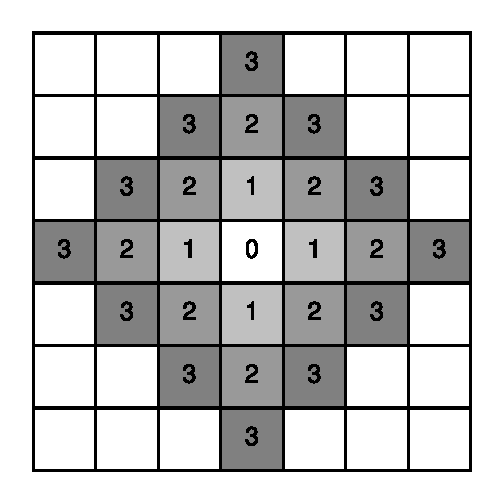
\includegraphics[width=\textwidth]{sources/max_manhattan/images/neighborhood}
	\caption[Cells in the Manhattan neighborhood of size $3$.]{Cells in the Manhattan neighborhood of size $3$. 
	The numbers in each cell represent the Manhattan distance from the central cell.}
	\label{fig:max_manhattan:neighborhood}
\end{figure}
This approach is clearly correct, and has a time complexity of $O(nmK^2)$. The space complexity is $O(1)$ as no additional space is used. 


\lstinputlisting[language=c++, caption={Brute Force solution to the problem of finding the max cell within the manhattan neighborhood of size $K$.},label=list:max_manhattan:bruteforce]{sources/max_manhattan/max_manhattan_solution1.cpp}


\subsection{Dynamic Programming}
\label{max_manhattan:sec:DP}
%This problem can be solved easily using dynamic programming.
%DP recurrence:
%dp[k][i][j] = ans. for kth manhattan distance for element (i,j)
%dp[k+1][i][j] = max(dp[k][i-1][j], dp[k][i+1][j], dp[k][i][j-1], dp[k][i][j+1], dp[k][i][j] )
%Recurrence is easy to get once you draw the figure.